\documentclass{article}
\usepackage{graphics}
\usepackage{epsfig}
\usepackage{hhline}

% define some macros:
\newcommand{\munged}{{\tt munged}}
\newcommand{\srun}{{\tt srun}}
\newcommand{\scancel}{{\tt scancel}}
\newcommand{\squeue}{{\tt squeue}}
\newcommand{\scontrol}{{\tt scontrol}}
\newcommand{\sinfo}{{\tt sinfo}}
\newcommand{\slurmctld}{{\tt slurmctld}}
\newcommand{\slurmd}{{\tt slurmd}}

\title{SLURM: Simple Linux Utility for Resource Management\thanks{
This document was prepared as an account of work sponsored by an
agency of the United States Government.  Neither the United States
Government nor the University of California nor any of their
employees, makes any warranty, express or implied, or assumes any
legal liability or responsibility for the accuracy, completeness, or
usefulness of any information, apparatus, product, or process
disclosed, or represents that its use would not infringe privately
owned rights. Reference herein to any specific commercial product,
process, or service by trade name, trademark, manufacturer, or
otherwise, does not necessarily constitute or imply its endorsement,
recommendation, or favoring by the United States Government or the
University of California.  The views and opinions of authors expressed
herein do not necessarily state or reflect those of the United States
Government or the University of California, and shall not be used for
advertising or product endorsement purposes.
This work was performed under the auspices of the U. S. Department of
Energy by the University of California, Lawrence Livermore National
Laboratory under Contract No. W-7405-Eng-48.}}

\author{Morris Jette \and Mark Grondona}

% We cheat here to easily get the desired allignment 
\date{\{jette1,mgrondona\}@llnl.gov}

\begin{document}

\maketitle

\begin{abstract}
Simple Linux Utility for Resource Management (SLURM) is an open source,
fault-tolerant, and highly scalable cluster management and job 
scheduling system for Linux clusters of thousands of nodes.  Components 
include machine status, partition management, job management, scheduling 
and stream copy modules.  This paper presents a overview of the SLURM architecture and functionality.
\end{abstract}

\section{Overview}

SLURM\footnote{A tip of the hat to Matt Groening and creators of {\em Futurama},
where Slurm is the highly addictive soda-like beverage made from worm
excrement.} (Simple Linux Utility for Resource Management) 
is a resource management 
system suitable for use on Linux clusters, large and small.  After 
surveying\cite{Jette2002} resource managers available for Linux and finding 
none that were simple, highly scalable, and portable to different cluster 
architectures and interconnects, the authors set out to design a new system.

The result is a resource management system with the following general
characteristics:

\begin{itemize}
\item {\em Simplicity}: SLURM is simple enough to allow motivated end users
to understand its source code and add functionality.  The authors will 
avoid the temptation to add features unless they are of general appeal. 

\item {\em Open Source}: SLURM is available to everyone and will remain free. 
Its source code is distributed under the GNU General Public 
License\cite{GPL2002}.

\item {\em Portability}: SLURM is written in the C language, with a GNU 
{\em autoconf} configuration engine.  
While initially written for Linux, other UNIX-like operating systems 
should be easy porting targets.
SLURM also supports a {\em plug-in} mechanism, which permits a variety 
of different infrastructures to be easily supported. 
The SLURM configuration file specifies which set of plug-in modules 
should be used. 

\item {\em Interconnect independence}: SLURM supports UDP/IP based
communication and the Quadrics Elan3 interconnect.  Adding support for 
other interconnects, including topography constraints, is straightforward 
and will utilize the plug-in mechanism described above\footnote{SLURM 
presently requires the specification of interconnect at build time. 
It will be converted to a plug-in with the next version of SLURM.}.

\item {\em Scalability}: SLURM is designed for scalability to clusters of
thousands of nodes. The SLURM controller for a cluster with 1000 nodes 
occupies on the order of 2 MB of memory and excellent performance has 
been demonstrated. 
Jobs may specify their resource requirements in a variety of ways 
including requirements options and ranges, potentially permitting 
faster initiation than otherwise possible.

\item {\em Fault tolerance}: SLURM can handle a variety of failure modes
without terminating workloads, including crashes of the node running 
the SLURM controller. 
User jobs may be configured to continue execution despite the failure 
of one or more nodes on which they are executing. 
The user command controlling a job, {\tt srun}, may detach and reattach 
from the parallel tasks at any time. 
Nodes allocated to a job are available for reuse as soon as the allocated 
job(s) to that node terminate. If some nodes fail to complete job termination 
in a timely fashion due to hardware of software problems, only the 
scheduling of those tardy nodes will be effected.

\item {\em Secure}: SLURM employs crypto technology to authenticate 
users to services and services to each other with a variety of options 
available through the plug-in mechanism.  
SLURM does not assume that its networks are physically secure, 
but does assume that the entire cluster is within a single 
administrative domain with a common user base across the 
entire cluster.

\item {\em System administrator friendly}: SLURM is configured a 
simple configuration file and minimizes distributed state.  
Its configuration may be changed at any time without impacting running jobs. 
Heterogeneous nodes within a cluster may be easily managed.
Its interfaces are usable by scripts and its behavior is highly 
deterministic.

\end{itemize}

\subsection{What is SLURM?}

As a cluster resource manager, SLURM has three key functions.  First,
it allocates exclusive and/or non-exclusive access to resources 
(compute nodes) to users for 
some duration of time so they can perform work.  Second, it provides 
a framework for starting, executing, and monitoring work (normally a 
parallel job) on the set of allocated nodes.  Finally, it arbitrates 
conflicting requests for resources by managing a queue of pending work.

Users interact with SLURM through four command line utilities: 
\srun\ for submitting a job for execution and optionally controlling it
interactively, 
\scancel\ for early termination of a pending or running job, 
\squeue\ for monitoring job queues, and 
\sinfo\ for monitoring partition and overall system state.
System administrators perform privileged operations through an additional
command line utility: {\tt scontrol}.

The central controller daemon, {\tt slurmctld}, maintains the global state 
and directs operations.
Compute nodes simply run a \slurmd\ daemon (similar to a remote shell 
daemon) to export control to SLURM.  

\subsection{What SLURM is Not}

SLURM is not a comprehensive cluster administration or monitoring package.  
While SLURM knows the state of its compute nodes, it makes no attempt to put
this information to use in other ways, such as with a general purpose event
logging mechanism or a back-end database for recording historical state.
It is expected that SLURM will be deployed in a cluster with other 
tools performing those functions. 

SLURM is not a meta-batch system like Globus\cite{Globus2002}
or DPCS (Distributed Production Control System)\cite{DPCS2002}.  
SLURM supports resource management across a single cluster.

SLURM is not a sophisticated batch system.  
In fact, it was expressly designed to provide high-performance 
parallel job management while leaving scheduling decisions to an 
external entity. 
Its default scheduler implements First-In First-Out (FIFO). 
An external entity can establish a job's initial priority 
through a plug-in.
An external scheduler may also submit, signal, hold, reorder and 
terminate jobs via the API.


\subsection{Architecture}

\begin{figure}[tb]
\centerline{\epsfig{file=figures/arch.eps,scale=1.2}}
\caption{SLURM Architecture}
\label{arch}
\end{figure}

As depicted in Figure~\ref{arch}, SLURM consists of a \slurmd\ daemon
running on each compute node, a central \slurmctld\ daemon running on
a management node (with optional fail-over twin), and five command line
utilities: {\tt srun}, {\tt scancel}, {\tt sinfo}, {\tt squeue}, and 
{\tt scontrol}, which can run anywhere in the cluster.  

The entities managed by these SLURM daemons include {\em nodes}, the
compute resource in SLURM, {\em partitions}, which group nodes into
logical disjoint sets, {\em jobs}, or allocations of resources assigned
to a user for a specified amount of time, and {\em job steps}, which are
sets of (possibly parallel) tasks within a job.  
Jobs are allocated nodes within 
partitions until the resources (nodes) within that partition are exhausted. 
Once a job is assigned a set of nodes, the user is able to initiate
parallel work in the form of job steps in any configuration within the
allocation. For instance a single job step may be started which utilizes
all nodes allocated to the job, or several job steps may independently 
use a portion of the allocation.

\begin{figure}[tcb]
\centerline{\epsfig{file=figures/entities.eps,scale=0.6}}
\caption{SLURM Entities}
\label{entities}
\end{figure}

Figure~\ref{entities} further illustrates the interrelation of these
entities as they are managed by SLURM. The diagram shows a group of
compute nodes split into two partitions. Partition 1 is running one
job, with one job step utilizing the full allocation of that job.
The job in Partition 2 has only one job step using half of the original
job allocation.
That job might initiate additional job step(s) to utilize 
the remaining nodes of its allocation.

\begin{figure}[tb]
\centerline{\epsfig{file=figures/slurm-arch.eps,scale=0.5}}
\caption{SLURM Architecture - Subsystems}
\label{archdetail}
\end{figure}

Figure~\ref{archdetail} exposes the subsystems that are implemented
within the \slurmd\ and \slurmctld\ daemons.  These subsystems
are explained in more detail below.

\subsubsection{Slurmd}

\slurmd\ is a multi-threaded daemon running on each compute node and 
can be compared to a remote shell daemon:  
it waits for work, executes the work, returns status,
then waits for more work.  
Since it initiates jobs for other users, it must run as user {tt root}.
It also asynchronously exchanges node and job status with {\tt slurmctld}.  
The only job information it has at any given time pertains to its 
currently executing jobs.
\slurmd\ reads the common SLURM configuration file, {\tt /etc/slurm.conf},
and has five major components:

\begin{itemize}
\item {\em Machine and Job Status Services}:  Respond to controller 
requests for machine and job state information, and send asynchronous 
reports of some state changes (e.g. \slurmd\ startup) to the controller.

\item {\em Remote Execution}: Start, monitor, and clean up after a set
of processes (typically belonging to a parallel job) as dictated by the
\slurmctld\ daemon or an \srun\ or \scancel\ command. Starting a process may
include executing a prolog program, setting process limits, setting real
and effective user id, establishing environment variables, setting working
directory, allocating interconnect resources, setting core file paths,
initializing the Stream Copy Service, and managing
process groups. Terminating a process may include terminating all members
of a process group and executing an epilog program.

\item {\em Stream Copy Service}: Allow handling of stderr, stdout, and
stdin of remote tasks. Job input may be redirected from a file or files, a
\srun\ process, or /dev/null.  Job output may be saved into local files or
sent back to the \srun\ command. Regardless of the location of stdout/err,
all job output is locally buffered to avoid blocking local tasks.

\item {\em Job Control}: Allow asynchronous interaction with the
Remote Execution environment by propagating signals or explicit job
termination requests to any set of locally managed processes.

\end{itemize}

\subsubsection{Slurmctld}

Most SLURM state information exists in the controller, {\tt slurmctld}.
\slurmctld\ is multi-threaded with independent read and write locks 
for the various data structures to enhance scalability. 
When \slurmctld\ starts, it reads the SLURM configuration file.  
It also can read additional state information
from a checkpoint file generated by a previous execution of {\tt slurmctld}.
Full controller state information is written to 
disk periodically with incremental changes written to disk immediately
for fault tolerance.  
\slurmctld\ runs in either master or standby mode, depending on the
state of its fail-over twin, if any.
\\slurmctld\ need not execute as user {\tt root}. 
In fact, it is recommended that a unique user entry be created for 
executing \slurmctld\ and that user must be identified in the SLURM 
configuration file as {\tt SlurmUser}.
\slurmctld\ has three major components:

\begin{itemize}
\item {\em Node Manager}: Monitors the state of each node in
the cluster.  It polls {\tt slurmd}'s for status periodically and
receives state change notifications from \slurmd\ daemons asynchronously.
It ensures that nodes have the prescribed configuration before being 
considered available for use.

\item {\em Partition Manager}: Groups nodes into non-overlapping sets called
{\em partitions}. Each partition can have associated with it various job
limits and access controls.  The partition manager also allocates nodes
to jobs based upon node and partition states and configurations. Requests
to initiate jobs come from the Job Manager.  \scontrol\ may be used
to administratively alter node and partition configurations.

\item {\em Job Manager}: Accepts user job requests and places pending 
jobs in a priority ordered queue. 
The Job Manager is awakened on a periodic basis and whenever there
is a change in state that might permit a job to begin running, such
as job completion, job submission, partition {\em up} transition,
node {\em up} transition, etc.  The Job Manager then makes a pass
through the priority ordered job queue. The highest priority jobs 
for each partition are allocated resources as possible. As soon as an 
allocation failure occurs for any partition, no lower-priority jobs for 
that partition are considered for initiation. 
After completing the scheduling cycle, the Job Manager's scheduling
thread sleeps.  Once a job has been allocated resources, the Job Manager
transfers necessary state information to those nodes, permitting it 
to commence execution.  When the Job Manager detects that
all nodes associated with a job have completed their work, it initiates
clean-up and performs another scheduling cycle as described above.

\end{itemize}

\subsubsection{Command Line Utilities}

The command line utilities are the user interface to SLURM functionality.
They offer users access to remote execution and job control. They also 
permit administrators to dynamically change the system configuration. The 
utilities read the global configuration file
to determine the host(s) for \slurmctld\ requests, and the ports for 
both for \slurmctld\ and \slurmd\ requests. 

\begin{itemize}
\item {\tt scancel}: Cancel a running or a pending job or job step, 
subject to authentication and authorization. This command can also 
be used to send an arbitrary signal to all processes on all nodes 
associated with a job or job step.

\item {\tt scontrol}: Perform privileged administrative commands
such as draining a node or partition in preparation for maintenance. 
Many \scontrol\ functions can only be executed by privileged users.

\item {\tt sinfo}: Display a summary of partition and node information.

\item {\tt squeue}: Display the queue of running and waiting jobs 
and/or job steps. A wide assortment of filtering, sorting, and output 
format options are available.

\item {\tt srun}: Allocate resources, submit jobs to the SLURM queue,
and initiate parallel tasks (job steps). 
Every set of executing parallel tasks has an associated \srun\ which 
initiated it and, if the \srun\ persists, managing it. 
Jobs may be submitted for later execution (e.g. batch), in which case 
\srun\ terminates after job submission. 
Jobs may also be submitted for interactive execution, where \srun\ keeps 
running to shepherd the running job. In this case, 
\srun\ negotiates connections with remote {\tt slurmd}'s 
for job initiation and to
get stdout and stderr, forward stdin\footnote{\srun\ command
line options select the stdin handling method such as broadcast to all
tasks, or send only to task 0.}, and respond to signals from the user.
\srun\ may also be instructed to allocate a set of resources and
spawn a shell with access to those resources.

\end{itemize}

\subsubsection{Communications Layer}

SLURM presently uses Berkeley sockets for communications. 
However, we anticipate using the plug-in mechanism to easily 
permit use of other communications layers. 
At LLNL we are using an Ethernet for SLURM communications and 
the Quadrics Elan switch exclusively for user applications. 
The SLURM configuration file permits the identification of each 
node's name to be used for communications as well as its hostname. 
In the case of a control machine known as {\em mcri} to be communicated 
with using the name {\em emcri}, this is represented in the 
configuration file as {\em ControlMachine=mcri ControlAddr=emcri}.
The name used for communication is the same as the hostname unless 
otherwise specified.

While SLURM is able to manage 1000 nodes without difficulty using 
sockets and Ethernet, we are reviewing other communication 
mechanisms which may offer improved scalability. 
One possible alternative is STORM\cite{STORM2001}. 
STORM uses the cluster interconnect and Network Interface Cards to 
provide high-speed communications including a broadcast capability. 
STORM only supports the Quadrics Elan interconnnect at present, 
but does offer the promise of improved performance and scalability. 

Internal SLURM functions pack and unpack data structures in machine 
independent format. We considered the use of XML style messages, 
but felt this would adversely impact performance (albeit slightly). 
If XML support is desired, it is straightforward to perform a translation 
and use the SLURM API's.

\subsubsection{Security}

SLURM has a simple security model: 
Any user of the cluster may submit parallel jobs to execute and cancel
his own jobs.  Any user may view SLURM configuration and state
information.  
Only privileged users may modify the SLURM configuration,
cancel any job, or perform other restricted activities.  
Privileged users in SLURM include the users {\tt root} 
and {\tt SlurmUser} (as defined in the SLURM configuration file). 
If permission to modify SLURM configuration is 
required by others, set-uid programs may be used to grant specific
permissions to specific users.

We presently support three authentication mechanisms via plug-ins: 
{\tt authd}\cite{Authd2002}, {\tt munged} and {\tt none} 
(ie. trust message contents). 
A plug-in can easily be developed for Kerberos or authentication 
mechanisms as desired.
The \munged\ implementation is described below.
A \munged\ daemon running as user {\tt root} on each node confirms the 
identify of the user making the request using the {\em getpeername} 
function and generates a credential. 
The credential contains a user id, 
group id, time-stamp, lifetime, some pseudo-random information, and 
any user supplied information. \munged\ uses a private key to 
generate a Message Authentication Code (MAC) for the credential.
\munged\ then uses a public key to symmetrically encrypt 
the credential including the MAC. 
SLURM daemons and programs transmit this encrypted 
credential with communications. The SLURM daemon receiving the message 
sends the credential to \munged\ on that node. 
\munged\ decrypts the credential using its private key, validates it 
and returns the user id and group id of the user originating the 
credential.
\munged\ prevents replay of a credential on any single node 
by recording credentials that have already been authenticated.
In SLURM's case, the user supplied information includes node 
identification information to prevent a credential from being 
used on nodes it is not destined for.

When resources are allocated to a user by the controller, a ``job 
step credential'' is generated by combining the user id, job id, 
step id, the list of resources allocated (nodes), and the credential
lifetime. This ``job step credential'' is encrypted with 
a \slurmctld\ private key. This credential 
is returned to the requesting agent ({\tt srun}) along with the
allocation response, and must be forwarded to the remote {\tt slurmd}'s 
upon job step initiation. \slurmd\ decrypts this credential with the
\slurmctld 's public key to verify that the user may access
resources on the local node. \slurmd\ also uses this ``job step credential'' 
to authenticate standard input, output, and error communication streams. 

Access to partitions may be restricted via a ``RootOnly'' flag.  
If this flag is set, job submit or allocation requests to this 
partition are only accepted if the effective user ID originating 
the request is a privileged user. 
The request from such a user may submit a job as any other user. 
This may be used, for example, to provide specific external schedulers
with exclusive access to partitions.  Individual users will not be 
permitted to directly submit jobs to such a partition, which would 
prevent the external scheduler from effectively managing it.  
Access to partitions may also be restricted to users who are 
members of specific Unix groups using a ``AllowGroups'' specification.

\subsection{Example:  Executing a Batch Job}

In this example a user wishes to run a job in batch mode, in which \srun\ returns 
immediately and the job executes ``in the background'' when resources
are available.
The job is a two-node run of script containing {\em mping}, a simple MPI application.
The user submits the job:
\begin{verbatim}
srun --batch --nodes 2 --nprocs 2 myscript
\end{verbatim}
The script {\em myscript} contains:
\begin{verbatim}
#!/bin/sh
srun hostname
mping 1 1048576
\end{verbatim}

The \srun\ command authenticates the user to the controller and submits
the job request. 
The request includes the \srun\ environment, current working directory, 
and command line option information. By default, stdout and stderr are
sent to files in the current working directory and stdin is copied from
{\tt /dev/null}.

The controller consults the partition manager to test whether the job 
will ever be able to run.  If the user has requested a non-existent partition,
more nodes than are configured in the partition, a non-existent constraint, 
etc., the partition manager returns an error and the request is discarded.
The failure is reported to \srun\ which informs the user and exits, for example:
\begin{verbatim}
srun: error: Unable to allocate resources: Invalid partition name
\end{verbatim}

On successful submission, the controller assigns the job a unique 
{\em slurm id}, adds it to the job queue and returns the job's
slurm id to \srun\, which reports this to user and exits, returning
success to the user's shell:

\begin{verbatim}
srun: jobid 42 submitted
\end{verbatim}

The controller awakens the Job Manager which tries to run
jobs starting at the head of the priority ordered job queue.  
It finds job {\em 42}
and makes a successful request to the partition manager to allocate 
two nodes from the default (or requested) partition: {\em dev6} and 
{\em dev7}.

The Job Manager then sends a request to the \slurmd\ on the first node 
in the job {\em dev6} to execute the script specified on user's
command line\footnote{Had the user specified an executable file rather 
than a job script, an \srun\ program would be initiated on the first 
node and \srun\ would initiate the executable with the desired task distribution.}.
The Job Manager also sends a 
copy of the environment, current working directory, stdout and stderr location,
along with other options. Additional environment variables are appended
to the user's environment before it is sent to the remote \slurmd\ detailing
the job's resources, such as the slurm job id ({\em 42}) and the
allocated nodes ({\em dev[6-7]}).

The remote \slurmd\ establishes the new environment, executes a SLURM 
prolog program (if one is configured) as user {\tt root}, and executes the
job script (or command) as the submitting user. The \srun\ within the job script 
detects that it is running with allocated resources from the presence
of the {\tt SLURM\_JOBID} environment variable. \srun\ connects to
\slurmctld\ to request a ``job step'' to run on all nodes of the current
job. \slurmctld\ validates the request and replies with a job credential
and switch resources. \srun\ then contacts \slurmd 's running on both
{\em dev6} and {\em dev7}, passing the job credential, environment,
current working directory, command path and arguments, and interconnect
information. The {\tt slurmd}'s verify the valid job credential, connect
stdout and stderr back to \srun , establish the environment, and execute
the command as the submitting user.

Unless instructed otherwise by the user, stdout and stderr are
copied to files in the current working directory by \srun :

\begin{verbatim}
/path/to/cwd/slurm-42.out
/path/to/cwd/slurm-42.err
\end{verbatim}

The user may examine the output files at any time if they reside 
in a globally accessible directory. In this example
{\tt slurm-42.out} would  contain the output of the job script's two 
commands (hostname and mping):

\begin{verbatim}
dev6
dev7
  1 pinged   0:        1 bytes      5.38 uSec     0.19 MB/s                     
  1 pinged   0:        2 bytes      5.32 uSec     0.38 MB/s                     
  1 pinged   0:        4 bytes      5.27 uSec     0.76 MB/s                     
  1 pinged   0:        8 bytes      5.39 uSec     1.48 MB/s                     
  ...
  1 pinged   0:  1048576 bytes   4682.97 uSec   223.91 MB/s              
\end{verbatim}

When the tasks complete execution, \srun\ is notified by \slurmd\ of each
task's exit status. \srun\ reports job step completion to the Job Manager
and exits. 
\slurmd\ detects when the job script terminates and notifies
the Job Manager of its exit status and begins cleanup. 
The Job Manager directs the {\tt slurmd}'s formerly assigned to the
job to run the SLURM epilog program (if one is configured) as user 
{\tt root}. 
Finally, the Job Manager releases the resources allocated to job {\em 42}
and updates the job status to {\em complete}. The record of a job's
existence is eventually purged.

\subsection{Example:  Executing an Interactive Job}

In this example a user wishes to run the same {\em mping} command 
in interactive mode, in which \srun\ blocks while the job executes 
and stdout/stderr of the job are copied onto stdout/stderr of {\tt srun}.
The user submits the job, this time without the {\tt batch} option:
\begin{verbatim}
srun --nodes 2 --nprocs 2 mping 1 1048576
\end{verbatim}

The \srun\ command authenticates the user to the controller and
makes a request for a resource allocation {\em and} job step. The Job Manager
responds with a list of nodes, a job credential, and interconnect
resources on successful allocation. If resources are not immediately
available, the request terminates or blocks depending upon user
options.

If the request is successful, \srun\ forwards the job run request
to the assigned \slurmd~'s in the same manner as the \srun\ in the
batch job script. In this case, the user sees the program output on 
stdout of {\tt srun}:

\begin{verbatim}
  1 pinged   0:        1 bytes      5.38 uSec     0.19 MB/s                     
  1 pinged   0:        2 bytes      5.32 uSec     0.38 MB/s                     
  1 pinged   0:        4 bytes      5.27 uSec     0.76 MB/s                     
  1 pinged   0:        8 bytes      5.39 uSec     1.48 MB/s                     
  ...
  1 pinged   0:  1048576 bytes   4682.97 uSec   223.91 MB/s              
\end{verbatim}

When the job terminates, \srun\ receives an EOF on each stream and
closes it, then receives the task exit status from each {\tt slurmd}.
The \srun\ process notifies \slurmctld\ that the job is complete 
and terminates. The controller contacts all \slurmd 's allocated to the
terminating job and issues a request to run the SLURM epilog, then releases
the job's resources.

If a signal is received by \srun\ while the job is executing (for example,
a SIGINT resulting from a Control-C), it is sent to each \slurmd\ which 
terminates the individual tasks and reports this to the job status manager,
which cleans up the job.

\subsection{Scheduling Infrastructure}

Scheduling parallel computers is a very complex matter.  
Several good public domain schedulers exist with the most 
popular being the Maui Scheduler\cite{Jackson2001,Maui2002}. 
The scheduler used at our site, DPCS\cite{DPCS2002}, is quite 
sophisticated and has over 150,000 lines of code. 
We felt no need to address scheduling issues within SLURM, but 
have instead developed a resource manager with a rich set of 
application programming interfaces (APIs) and the flexibility 
to satisfy the needs of others working on scheduling issues.  

When jobs are submitted to SLURM they are assigned an initial 
scheduling priority through a plug-in library function. It 
maintains a priority ordered queue of pending jobs

to perform gang scheduling, namely an API 
to explicit preempt and later resume a job.

\section{Results}

\begin{figure}[htb]
\centerline{\epsfig{file=figures/times.eps}}
\caption{Time to execute /bin/hostname with various node counts}
\label{timing}
\end{figure}

We were able to perform some SLURM tests on a 1000 node cluster in 
November 2002. Some development was still underway at that time and 
tuning had not been performed. The results for executing the program 
{\em /bin/hostname} on two tasks per node and various node counts is show 
in Figure~\ref{timing}. We found SLURM performance to be comparable 
to the Quadrics Resource Management System (RMS)\cite{Quadrics2002} 
for all job sizes and about 80 times faster than IBM 
LoadLeveler\cite{LL2002} at small job sizes.
(While not shown on this chart, LoadLeveler reaches 1200 seconds to 
launch an 8000 task job on 500 nodes.)

\section{Future plans}

We expect SLURM to begin production use on LLNL Linux clusters 
starting in March 2003 and be available for distribution shortly 
thereafter. 

Looking ahead, we anticipate moving the interconnect topography 
and API functions into plug-in modules and adding support for 
additional systems. 
We plan to add support for additional operating systems 
(IA64 and x86-64) and interconnects (InfiniBand, Myrinet, and 
the IBM Blue Gene\cite{BlueGene2002} system\footnote{Blue Gene 
has a different interconnect than any supported by SLURM and 
a 3-D topography with restrictive allocation constraints.}). 
We plan to add support for suspending and resuming jobs, which 
provides the infrastructure needed to support gang scheduling. 
We also plan to support changing the node count associated 
with running jobs (as needed for MPI2). 
Recording resource use by each parallel job is planned for a 
future release.

\bibliographystyle{plain}
\bibliography{project}

\end{document}
